% --- IMPORTS ---
\documentclass[leqno]{article}
\usepackage{graphicx}
\usepackage{dsfont}
\usepackage{mathtools}
\usepackage{amssymb}
\usepackage{amsmath}
\usepackage{amsthm}
\usepackage{float}
\usepackage{ragged2e}
\usepackage{tensor}
\usepackage{fancyhdr}
\usepackage{empheq}
\usepackage[most]{tcolorbox}
\usepackage{enumitem}
\usepackage{dirtytalk}
\usepackage{marginnote}
\usepackage{microtype}
\usepackage[
  a4paper,
  left=0.8in,
  right=1in,
  top=1in,
  bottom=0.5in,
  headheight=14pt,
  headsep=0.4in
]{geometry}
\setlength{\parindent}{0cm}
% --- TikZ Packages ---
\usepackage{pgfplots}
\pgfplotsset{compat=1.18}
\usepgfplotslibrary{fillbetween, polar}
\usetikzlibrary{calc, positioning}
\usetikzlibrary{angles, quotes}
\usetikzlibrary{arrows.meta}
\usetikzlibrary{decorations.pathreplacing, decorations.markings}
\usetikzlibrary{patterns}
\usetikzlibrary{intersections}
% --- URL Packages ---
\usepackage[colorlinks=true,linkcolor=red,citecolor=magenta,urlcolor=black]{hyperref}%
\urlstyle{same}
% --- END OF IMPORTS ---

% --- CUSTOM COMMANDS ---
\RenewDocumentCommand{\marks}{o m}{%
  \IfValueTF{#1}%
    {\marginnote{\raggedright\textbf{[#2]}}[#1]}%
    {\marginnote{\raggedright\textbf{[#2]}}}%
}
\newcommand{\vspacerule}[2]{%
  \par\vspace*{#1}%
  \noindent\hrulefill\par
  \vspace*{#2}%
}
\definecolor{scarlet}{RGB}{205, 40, 75}
\newcommand{\questionitem}{%
  \item\phantomsection
  \addcontentsline{toc}{section}{Question \number\value{enumi}}%
}
\renewcommand{\contentsname}{Questions}
% --- END OF CUSTOM COMMANDS ---

% --- HEADER CONFIG ---
\pagestyle{fancy}
\fancyhead{}
\fancyfoot{}
\renewcommand{\headrulewidth}{0.9pt}
\lhead{\textit{Solutions} - Modelling with 2nd Order Differential Equations}
\chead{}
\rhead{\href{https://danieljsmith.org}{danieljsmith.org}}
% --- END OF HEADER CONFIG ---

\begin{document}
\vspace*{20pt}
\tableofcontents
\newpage
\begin{enumerate}[
  label=\textbf{\arabic*.},
  leftmargin=*,
  topsep=0pt,
  partopsep=0pt,
  parsep=0pt
]

% ---- Question 1 ----
\questionitem
% [Source: _QBT___Solns__Modelling_with_2nd_Order_Differential_Equations, Q1]

\begin{figure}[H]
    \centering
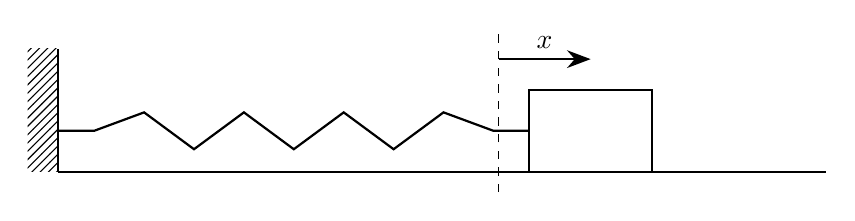
\begin{tikzpicture}[scale=1.3]
\def\wallx{-3.2}
\def\eqx{1.1}
\def\disp{0.9}
\def\bw{1.2}
\def\bh{0.8}
\pgfmathsetmacro{\midy}{\bh/2}
\pgfmathsetmacro{\cx}{\eqx+\disp}
\pgfmathsetmacro{\leftx}{\cx-\bw/2}
\pgfmathsetmacro{\rightx}{\cx+\bw/2}
\pgfmathsetmacro{\lead}{0.35}
\pgfmathsetmacro{\amp}{0.18}
\pgfmathsetmacro{\coilstart}{\wallx+\lead}
\pgfmathsetmacro{\coilend}{\leftx-\lead}
\pgfmathsetmacro{\step}{(\coilend-\coilstart)/8}
\pgfmathsetmacro{\arrowy}{\bh+0.3}
\pgfmathsetmacro{\marktop}{\bh+0.55}

\fill[pattern=north east lines] (\wallx-0.3,0) rectangle (\wallx,1.2);
\draw[thick] (\wallx,0) -- (\wallx,1.2);
\draw[thick] (\wallx,0) -- (4.3,0);

\draw[thick] (\wallx,\midy) -- (\coilstart,\midy)
  -- ++(\step,\amp) -- ++(\step,{-2*\amp}) -- ++(\step,{2*\amp})
  -- ++(\step,{-2*\amp}) -- ++(\step,{2*\amp}) -- ++(\step,{-2*\amp})
  -- ++(\step,{2*\amp}) -- ++(\step,{-\amp}) -- (\leftx,\midy);

\draw[thick] (\leftx,0) rectangle (\rightx,\bh);
\draw[dashed] (\eqx,-0.2) -- (\eqx,\marktop);
\draw[-{Stealth[length=3mm]}, thick] (\eqx,\arrowy) -- (\cx,\arrowy) node[midway, above] {$x$};
\end{tikzpicture}
\end{figure}


The horizontal displacement of a glider attached to a spring, shown in the diagram above, is modelled by the differential equation \\
\[\frac{\mathrm{d}^2 x}{\mathrm{d} t^2}+16x=3\sin 4t\] \\
where $x$ is the displacement, in metres, of the glider from its equilibrium position, $t$ seconds after the motion begins. \\
\begin{enumerate}[label=\textbf{(\alph*)}]
  \item
  \begin{enumerate}[label=(\roman*)]
    \item Show that a particular solution of the differential equation is
    \[
    x=-\frac{3}{8} t \cos 4t
    \] \marks[-20pt]{4}
    \item Hence, find the general solution of the differential equation \marks{4} \\
  \end{enumerate}
\end{enumerate}
Initially, the glider is $0.20\,\mathrm{m}$ to the right of equilibrium and is moving towards equilibrium at $0.50\,\mathrm{m\,s^{-1}}$. \\
Given that, $4$ seconds after the motion begins, the displacement of the glider is $\beta$ m, \\
\begin{enumerate}[label=\textbf{(\alph*)}, resume]
  \item determine, according to the model, the value of $\beta$ to $3$ significant figures \marks{4} \\
  \item Given that the true value of $\beta$ is $0.46\,\mathrm{m}$, comment on the suitability of the model \marks{1} \\
  \item Write down a differential equation for the glider if the periodic driving force is removed, so that the motion becomes simple harmonic \marks{1} \\
\end{enumerate}

\vspace*{10pt}

\begin{tcolorbox}[colback=white, colframe=scarlet, title={\textbf{Solution}}, breakable, grow to left by=6mm, grow to right by=10mm]
\begin{enumerate}[label=\textbf{(\alph*)}]
  \item
  \begin{enumerate}[label=(\roman*)]
    \item The corresponding homogeneous equation is
    \[
    \frac{\mathrm{d}^2x}{\mathrm{d}t^2}+16x=0
    \]
    whose solutions involve $\cos 4t$ and $\sin 4t$.

    Since the forcing term is $3\sin 4t$, the usual trial $A\cos 4t+B\sin 4t$ would duplicate the complementary function, so we try
    \[
    x_p=t(A\cos 4t+B\sin 4t)
    \]

    Differentiate:
    \begin{align*}
    \frac{\mathrm{d}x_p}{\mathrm{d}t}
    &= (A\cos 4t+B\sin 4t)+t(-4A\sin 4t+4B\cos 4t) \\
    &= A\cos 4t+B\sin 4t-4At\sin 4t+4Bt\cos 4t
    \end{align*}

    Differentiate again:
    \begin{align*}
    \frac{\mathrm{d}^2x_p}{\mathrm{d}t^2}
    &= -4A\sin 4t+4B\cos 4t-4A\sin 4t-16At\cos 4t+4B\cos 4t-16Bt\sin 4t \\
    &= -8A\sin 4t+8B\cos 4t-16At\cos 4t-16Bt\sin 4t
    \end{align*}

    Substitute into the differential equation:
    \begin{align*}
    \frac{\mathrm{d}^2x_p}{\mathrm{d}t^2}+16x_p
    &= \left(-8A\sin 4t+8B\cos 4t-16At\cos 4t-16Bt\sin 4t\right) \\
    &\quad +16t(A\cos 4t+B\sin 4t) \\
    &= -8A\sin 4t+8B\cos 4t
    \end{align*}

    For this to equal $3\sin 4t$, we compare coefficients:
    \[
    -8A=3,\qquad 8B=0
    \]

    Hence
    \[
    A=-\frac{3}{8},\qquad B=0
    \]

    So a particular solution is
    \[
    x_p=-\frac{3}{8}t\cos 4t
    \]

    \item The complementary function $x_c$ comes from
    \[
    \lambda^2+16=0
    \]
    so
    \[
    \lambda=\pm 4i
    \]

    Therefore
    \[
    x_c=C\cos 4t+D\sin 4t
    \]

    Hence the general solution is
    \[
    x=x_c+x_p=C\cos 4t+D\sin 4t-\frac{3}{8}t\cos 4t
    \]

    So the general solution is
    \[
    x=C\cos 4t+D\sin 4t-\frac{3}{8}t\cos 4t
    \]
  \end{enumerate}

  \item Using
  \[
  x=C\cos 4t+D\sin 4t-\frac{3}{8}t\cos 4t
  \]

  First use $x(0)=0.20$:
  \[
  0.20=C\cos 0+D\sin 0-\frac{3}{8}(0)\cos 0
  \]
  so
  \[
  C=0.20
  \]

  Differentiate $x$:
  \begin{align*}
  \frac{\mathrm{d}x}{\mathrm{d}t}
  &= -4C\sin 4t+4D\cos 4t-\frac{3}{8}\cos 4t+\frac{3}{2}t\sin 4t
  \end{align*}

  Initially the glider is to the right of equilibrium, and moving towards equilibrium, so its initial velocity is negative:
  \[
  \frac{\mathrm{d}x}{\mathrm{d}t}(0)=-0.50
  \]

  Substitute $t=0$:
  \[
  -0.50=-4C\sin 0+4D\cos 0-\frac{3}{8}\cos 0+\frac{3}{2}(0)\sin 0
  \]
  so
  \[
  -0.50=4D-\frac{3}{8}
  \]

  Hence
  \begin{align*}
  4D&=-\frac{1}{2}+\frac{3}{8} \\
     &=-\frac{1}{8}
  \end{align*}
  and therefore
  \[
  D=-\frac{1}{32}
  \]

  So the displacement is
  \[
  x=0.20\cos 4t-\frac{1}{32}\sin 4t-\frac{3}{8}t\cos 4t
  \]

  When $t=4$,
  \begin{align*}
  \beta=x(4)
  &=0.20\cos 16-\frac{1}{32}\sin 16-\frac{3}{8}(4)\cos 16 \\
  &=0.20\cos 16-\frac{1}{32}\sin 16-\frac{3}{2}\cos 16 \\
  &\approx 1.25
  \end{align*}

  Therefore
  \[
  \beta \approx 1.25\text{ m}
  \]
  to 3 significant figures.

  \item The model is not very suitable, since it predicts $\beta\approx 1.25$ m whereas the true value is $0.46$ m, so it overestimates the displacement by a large amount.

  \item With the periodic driving force removed, the right-hand side becomes $0$, so the differential equation is
  \[
  \frac{\mathrm{d}^2x}{\mathrm{d}t^2}+16x=0
  \]
\end{enumerate}
\end{tcolorbox}


\newpage

% ---- Question 2 ----
\questionitem
% [Source: _QBT___Solns__Modelling_with_2nd_Order_Differential_Equations, Q2]

\begin{figure}[H]
    \centering
\begin{tikzpicture}[scale=1.3]
\def\lineL{3.8}
\def\pos{2.6}
\def\velLen{1.25}
\def\forceLen{1.25}
\def\dispY{0.75}

\coordinate (O) at (0,0);
\coordinate (P) at (\pos,0);

\draw[thick, dashed] (-\lineL,0) -- (P);
\draw[thick] ($(O)+(0,-0.18)$) -- ($(O)+(0,0.18)$);
\node[above] at ($(O)+(0,0.15)$) {$O$};

\fill (P) circle (2.8pt);

\draw[-{Stealth[length=3mm]}, thick]
    ($(P)+(0.75,0.65)$) -- ++(-\velLen,0)
    node[midway, above, xshift=5pt] {$v\,\mathrm{m\,s^{-1}}$};

\draw[-{Stealth[length=3mm]}, thick]
    ($(P)+(1.50,0)$) -- ++(-\forceLen,0)
    node[midway, below, xshift=5pt] {$9mx\,\mathrm{N}$};

\draw[-{Stealth[length=3mm]}, thick]
    ($(O)+(0,-\dispY)$) -- ($(P)+(0,-\dispY)$)
    node[midway, below] {$x\,\mathrm{m}$};
\end{tikzpicture}
\end{figure}


A particle of mass $m\,\mathrm{kg}$ moves in a horizontal line through its equilibrium position $O$. At time $t$ seconds its displacement from $O$ is $x$ metres and its speed is $v\,\mathrm{m\,s^{-1}}$. When the particle is to the right of $O$, it is acted on by a restoring force of magnitude $9mx$ newtons directed towards $O$, as shown in the diagram. \\

At $t=0$, the particle is $1$ m to the right of $O$ and is projected towards $O$ with speed $6\,\mathrm{m\,s^{-1}}$. \\

\begin{enumerate}[label=\textbf{(\alph*)}]
  \item In the absence of damping and any external force,
  \begin{enumerate}[label=(\roman*)]
    \item Show that the motion is modelled by the differential equation
    \[
    \frac{\mathrm{d}^2 x}{\mathrm{d} t^2}+9x=0
    \] \marks[-20pt]{1}
    \item State the type of motion \marks{1}
    \item Write down the period of the motion \marks{1}
    \item Find $x$ in terms of $t$ \marks{4}
    \item Find the amplitude of the motion \marks{2} \\
  \end{enumerate}
  \item In a second model, the particle again starts from the same initial position and velocity, but the motion is damped by a force $6mv$ newtons acting opposite to the direction of motion. \\
  \begin{enumerate}[label=(\roman*)]
    \item Show that
    \[
    \frac{\mathrm{d}^2 x}{\mathrm{d} t^2}+6\frac{\mathrm{d} x}{\mathrm{d} t}+9x=0
    \] \marks[-20pt]{1}
    \item State, giving a reason, whether the system is under-damped, critically damped or over-damped \marks{1}
    \item Determine the general solution of this differential equation \marks{3} \\
  \end{enumerate}
  \item In a third model, the particle again starts from the same initial position and velocity, and is subject both to the damping force in part (b) and to an external force $25m\cos 4t$ newtons acting in the positive direction. The motion is now modelled by the differential equation
  \[
  \frac{\mathrm{d}^2 x}{\mathrm{d} t^2}+6\frac{\mathrm{d} x}{\mathrm{d} t}+9x=25\cos 4t
  \]
  \begin{enumerate}[label=(\roman*)]
    \item Find $x$ in terms of $t$ \marks{7} \\
    \item In the long term, the particle is observed to perform simple harmonic motion with period about $1.6$ seconds. Verify that this is consistent with the answer to part (c)(i) \marks{2} \\
  \end{enumerate}
\end{enumerate}

\vspace*{10pt}

\begin{tcolorbox}[colback=white, colframe=scarlet, title={\textbf{Solution}}, breakable, grow to left by=6mm, grow to right by=10mm]
\begin{enumerate}[label=\textbf{(\alph*)}]
  \item
  \begin{enumerate}[label=(\roman*)]
    \item Taking displacement to the right as positive, the restoring force is
    \[
    -9mx
    \]
    By Newton's second law,
    \[
    m\frac{\mathrm{d}^2x}{\mathrm{d}t^2}=-9mx
    \]
    Hence
    \[
    \frac{\mathrm{d}^2x}{\mathrm{d}t^2}+9x=0
    \]

    \item From part (i),
    \[
    \frac{\mathrm{d}^2x}{\mathrm{d}t^2}=-9x
    \]
    so the acceleration is proportional to the displacement and directed towards the equilibrium position. Therefore the motion is simple harmonic motion.

    \item For SHM,
    \[
    \omega^2=9
    \]
    so \(\omega=3\). Hence the period is
    \[
    T=\frac{2\pi}{\omega}=\frac{2\pi}{3}\text{ s}
    \]

    \item To solve
    \[
    \frac{\mathrm{d}^2x}{\mathrm{d}t^2}+9x=0
    \]
    the auxiliary equation is
    \[
    \lambda^2+9=0
    \]
    giving roots \(\lambda=\pm 3i\). So
    \[
    x=A\cos 3t+B\sin 3t
    \]
    Using \(x(0)=1\),
    \[
    1=A\cos 0+B\sin 0=A
    \]
    so \(A=1\).

    Differentiate:
    \[
    \frac{\mathrm{d}x}{\mathrm{d}t}=-3A\sin 3t+3B\cos 3t
    \]
    At \(t=0\), the particle is projected towards \(O\) with speed \(6\), so
    \[
    \frac{\mathrm{d}x}{\mathrm{d}t}(0)=-6
    \]
    Hence
    \[
    -6=-3A\sin 0+3B\cos 0=3B
    \]
    so \(B=-2\).

    Therefore
    \[
    x=\cos 3t-2\sin 3t
    \]

    \item For
    \[
    x=A\cos 3t+B\sin 3t
    \]
    the amplitude is
    \[
    \sqrt{A^2+B^2}
    \]
    Here \(A=1\) and \(B=-2\), so
    \[
    \text{Amplitude}=\sqrt{1^2+(-2)^2}=\sqrt{5}\text{ m}
    \]
  \end{enumerate}

  \item
  \begin{enumerate}[label=(\roman*)]
    \item The damping force has magnitude \(6mv\) and acts opposite to the motion, so in signed form it is
    \[
    -6m\frac{\mathrm{d}x}{\mathrm{d}t}
    \]
    The forces on the particle are therefore
    \[
    -6m\frac{\mathrm{d}x}{\mathrm{d}t}-9mx
    \]
    By Newton's second law,
    \[
    m\frac{\mathrm{d}^2x}{\mathrm{d}t^2}=-6m\frac{\mathrm{d}x}{\mathrm{d}t}-9mx
    \]
    Hence
    \[
    \frac{\mathrm{d}^2x}{\mathrm{d}t^2}+6\frac{\mathrm{d}x}{\mathrm{d}t}+9x=0
    \]

    \item The auxiliary equation is
    \[
    \lambda^2+6\lambda+9=0
    \]
    so
    \[
    (\lambda+3)^2=0
    \]
    There is a repeated real root, so the system is critically damped.

    \item Since the auxiliary equation has repeated root \(\lambda=-3\), the general solution is
    \[
    x=(A+Bt)e^{-3t}
    \]
  \end{enumerate}

  \item
  \begin{enumerate}[label=(\roman*)]
    \item We solve
    \[
    \frac{\mathrm{d}^2x}{\mathrm{d}t^2}+6\frac{\mathrm{d}x}{\mathrm{d}t}+9x=25\cos 4t
    \]

    From part (b), the complementary function is
    \[
    x_c=(A+Bt)e^{-3t}
    \]

    For a particular integral, try
    \[
    x_p=a\cos 4t+b\sin 4t
    \]
    Then
    \begin{align*}
    \frac{\mathrm{d}x_p}{\mathrm{d}t} &= -4a\sin 4t+4b\cos 4t \\
    \frac{\mathrm{d}^2x_p}{\mathrm{d}t^2} &= -16a\cos 4t-16b\sin 4t
    \end{align*}

    Substituting into the differential equation gives
    \begin{align*}
    &(-16a\cos 4t-16b\sin 4t)+6(-4a\sin 4t+4b\cos 4t)+9(a\cos 4t+b\sin 4t) \\
    &= 25\cos 4t
    \end{align*}
    so
    \[
    (-7a+24b)\cos 4t+(-24a-7b)\sin 4t=25\cos 4t
    \]
    Equating coefficients,
    \begin{align*}
    -7a+24b&=25 \\
    -24a-7b&=0
    \end{align*}

    From the second equation,
    \[
    24a+7b=0
    \]
    Solving the pair gives
    \[
    a=-\frac{7}{25}, \qquad b=\frac{24}{25}
    \]
    Hence
    \[
    x=(A+Bt)e^{-3t}-\frac{7}{25}\cos 4t+\frac{24}{25}\sin 4t
    \]

    Now use the initial conditions.

    Since \(x(0)=1\),
    \[
    A-\frac{7}{25}=1
    \]
    so
    \[
    A=\frac{32}{25}
    \]

    Differentiate \(x\):
    \begin{align*}
    \frac{\mathrm{d}x}{\mathrm{d}t}
    &= \frac{\mathrm{d}}{\mathrm{d}t}\left((A+Bt)e^{-3t}\right)+\frac{28}{25}\sin 4t+\frac{96}{25}\cos 4t \\
    &= \left(B-3A-3Bt\right)e^{-3t}+\frac{28}{25}\sin 4t+\frac{96}{25}\cos 4t
    \end{align*}

    Since the particle is initially projected towards \(O\) with speed \(6\),
    \[
    \frac{\mathrm{d}x}{\mathrm{d}t}(0)=-6
    \]
    Therefore
    \[
    B-3A+\frac{96}{25}=-6
    \]
    Substituting \(A=\frac{32}{25}\),
    \[
    B-3\left(\frac{32}{25}\right)+\frac{96}{25}=-6
    \]
    \[
    B=-6
    \]

    So
    \[
    x=\left(\frac{32}{25}-6t\right)e^{-3t}-\frac{7}{25}\cos 4t+\frac{24}{25}\sin 4t
    \]

    \item From part (i),
    \[
    x=\left(\frac{32}{25}-6t\right)e^{-3t}-\frac{7}{25}\cos 4t+\frac{24}{25}\sin 4t
    \]
    As \(t\to\infty\),
    \[
    \left(\frac{32}{25}-6t\right)e^{-3t}\to 0
    \]
    so the long-term motion is
    \[
    x=-\frac{7}{25}\cos 4t+\frac{24}{25}\sin 4t
    \]
    This is a sinusoidal function, so it is simple harmonic motion with angular frequency \(4\).

    Hence its period is
    \[
    T=\frac{2\pi}{4}=\frac{\pi}{2}\approx 1.57\text{ s}
    \]
    which is consistent with the observed period of about \(1.6\) s.
  \end{enumerate}
\end{enumerate}
\end{tcolorbox}


\newpage

% ---- Question 3 ----
\questionitem
% [Source: _QBT___Solns__Modelling_with_2nd_Order_Differential_Equations, Q3]

The charge $q$ on a capacitor in a driven RLC circuit is modelled by \\
\[\frac{\mathrm{d}^2 q}{\mathrm{d} t^2}+2\frac{\mathrm{d} q}{\mathrm{d} t}+10q=37\cos 3t\] \\
where $t\geq0$ is time. \\

When $t=0$, $q=1$ and $\frac{\mathrm{d} q}{\mathrm{d} t}=15$. \\

\begin{enumerate}[label=\textbf{(\alph*)}]
  \item Find $q$ as a function of $t$ \marks{9} \\
  \item Hence write down an approximate expression for $q$ when $t$ is large, giving your answer in the form $R\cos(3t-\alpha)$, where $R>0$ and $0<\alpha<\frac{\pi}{2}$ \marks{4} \\
\end{enumerate}

\vspace*{10pt}

\begin{tcolorbox}[colback=white, colframe=scarlet, title={\textbf{Solution}}, breakable, grow to left by=6mm, grow to right by=10mm]
\begin{enumerate}[label=\textbf{(\alph*)}]
  \item Solve
  \[
  \frac{\mathrm{d}^2q}{\mathrm{d}t^2}+2\frac{\mathrm{d}q}{\mathrm{d}t}+10q=37\cos 3t
  \]

  First find the complementary function from the homogeneous equation
  \[
  \frac{\mathrm{d}^2q}{\mathrm{d}t^2}+2\frac{\mathrm{d}q}{\mathrm{d}t}+10q=0
  \]

  The auxiliary equation is
  \[
  \lambda^2+2\lambda+10=0
  \]

  Solving,
  \begin{align*}
  \lambda&=\frac{-2\pm\sqrt{2^2-4(1)(10)}}{2} \\
  &=\frac{-2\pm\sqrt{-36}}{2} \\
  &=\frac{-2\pm 6\mathrm{i}}{2} \\
  &=-1\pm 3\mathrm{i}
  \end{align*}

  Hence the complementary function is
  \[
  e^{-t}(A\cos 3t+B\sin 3t)
  \]

  For a particular integral, since the forcing term is \(37\cos 3t\), try
  \[
  q_p=a\cos 3t+b\sin 3t
  \]

  Then
  \begin{align*}
  \frac{\mathrm{d}q_p}{\mathrm{d}t}&=-3a\sin 3t+3b\cos 3t \\
  \frac{\mathrm{d}^2q_p}{\mathrm{d}t^2}&=-9a\cos 3t-9b\sin 3t
  \end{align*}

  Substituting into the differential equation:
  \begin{align*}
  &(-9a\cos 3t-9b\sin 3t)+2(-3a\sin 3t+3b\cos 3t)+10(a\cos 3t+b\sin 3t) \\
  &=37\cos 3t
  \end{align*}

  Collecting \(\cos 3t\) and \(\sin 3t\) terms:
  \begin{align*}
  (-9a+6b+10a)\cos 3t+(-9b-6a+10b)\sin 3t&=37\cos 3t \\
  (a+6b)\cos 3t+(b-6a)\sin 3t&=37\cos 3t
  \end{align*}

  Equating coefficients gives
  \begin{align*}
  a+6b&=37 \\
  b-6a&=0
  \end{align*}

  From \(b=6a\), substitute into the first equation:
  \begin{align*}
  a+6(6a)&=37 \\
  37a&=37 \\
  a&=1
  \end{align*}

  So
  \[
  b=6
  \]

  Therefore the general solution is
  \[
  q=e^{-t}(A\cos 3t+B\sin 3t)+\cos 3t+6\sin 3t
  \]

  Now use the initial conditions.

  When \(t=0\), \(q=1\):
  \begin{align*}
  1&=e^{0}(A\cos 0+B\sin 0)+\cos 0+6\sin 0 \\
  1&=A+1
  \end{align*}

  Hence
  \[
  A=0
  \]

  Differentiate the general solution:
  \begin{align*}
  \frac{\mathrm{d}q}{\mathrm{d}t}
  &=\frac{\mathrm{d}}{\mathrm{d}t}\left[e^{-t}(A\cos 3t+B\sin 3t)\right]-3\sin 3t+18\cos 3t \\
  &=e^{-t}\left[(-A\cos 3t-B\sin 3t)+(-3A\sin 3t+3B\cos 3t)\right]-3\sin 3t+18\cos 3t \\
  &=e^{-t}\left[(3B-A)\cos 3t+(-3A-B)\sin 3t\right]-3\sin 3t+18\cos 3t
  \end{align*}

  When \(t=0\), \(\frac{\mathrm{d}q}{\mathrm{d}t}=15\):
  \begin{align*}
  15&=e^{0}\left[(3B-A)\cos 0+(-3A-B)\sin 0\right]-3\sin 0+18\cos 0 \\
  15&=3B-A+18
  \end{align*}

  Since \(A=0\),
  \begin{align*}
  15&=3B+18 \\
  3B&=-3 \\
  B&=-1
  \end{align*}

  So
  \[
  q=e^{-t}(0\cdot \cos 3t-\sin 3t)+\cos 3t+6\sin 3t
  \]

  Hence
  \[
  q=\cos 3t+6\sin 3t-e^{-t}\sin 3t
  \]

  Therefore,
  \[
  q(t)=\cos 3t+6\sin 3t-e^{-t}\sin 3t
  \]

  \item For large \(t\), the term \(e^{-t}\sin 3t\to 0\), so
  \[
  q\approx \cos 3t+6\sin 3t
  \]

  Write this in the form \(R\cos(3t-\alpha)\). Using
  \[
  \cos(3t-\alpha)=\cos 3t\cos\alpha+\sin 3t\sin\alpha
  \]

  we have
  \[
  R\cos(3t-\alpha)=R\cos\alpha\cos 3t+R\sin\alpha\sin 3t
  \]

  Comparing coefficients with \(\cos 3t+6\sin 3t\),
  \begin{align*}
  R\cos\alpha&=1 \\
  R\sin\alpha&=6
  \end{align*}

  Squaring and adding:
  \begin{align*}
  R^2\cos^2\alpha+R^2\sin^2\alpha&=1^2+6^2 \\
  R^2(\cos^2\alpha+\sin^2\alpha)&=37 \\
  R^2&=37
  \end{align*}

  Since \(R>0\),
  \[
  R=\sqrt{37}
  \]

  Also,
  \[
  \tan\alpha=\frac{R\sin\alpha}{R\cos\alpha}=\frac{6}{1}=6
  \]

  so
  \[
  \alpha=\arctan 6
  \]

  Therefore the large-\(t\) approximation is
  \[
  q\approx \sqrt{37}\cos(3t-\arctan 6)
  \]

  Numerically, this is
  \[
  q\approx 6.08\cos(3t-1.41)
  \]
\end{enumerate}
\end{tcolorbox}


\newpage

% ---- Question 4 ----
\questionitem
% [Source: _QBT___Solns__Modelling_with_2nd_Order_Differential_Equations, Q4]

The vertical displacement of the body of a car from its steady running height is measured by $y$ metres, where $y$ is positive upwards. The body can move above or below this level, so $y$ can take positive and negative values. After the car leaves a speed hump, the body is momentarily above its steady running height and at rest at time $t=0$. \\

A proposed model for the subsequent motion, for $t\ge 0$, is
\[
4\frac{\mathrm{d}^2 y}{\mathrm{d} t^2}+p\frac{\mathrm{d} y}{\mathrm{d} t}+9y=0,
\]
where $p$ is a constant and $p\ge 0$. \\

\begin{enumerate}[label=\textbf{(\alph*)}]
  \item
  \begin{enumerate}[label=(\roman*)]
    \item According to the model, for what value of $p$ would the motion be simple harmonic? \marks{1}
    \item Explain briefly why modelling the motion as simple harmonic is unlikely to be realistic for a car suspension \marks{1} \\
  \end{enumerate}
  \item Find the range of values of $p$ for which the model predicts that the body of the car never goes below its steady running height \marks{2} \\
  \item Sketch a possible graph of $y$ against $t$ when $p$ lies outside the range found in part (b) but the motion is not simple harmonic \marks{1} \\
\end{enumerate}

\vspace*{10pt}

\begin{tcolorbox}[colback=white, colframe=scarlet, title={\textbf{Solution}}, breakable, grow to left by=6mm, grow to right by=10mm]
\begin{enumerate}[label=\textbf{(\alph*)}]
  \item
  \begin{enumerate}[label=(\roman*)]
    \item For simple harmonic motion there is no damping term, so the coefficient of $\dfrac{\mathrm{d}y}{\mathrm{d}t}$ must be zero.

    \[
    p=0
    \]

    So the motion is simple harmonic when $p=0$.

    \item In a real car suspension there is damping, due to shock absorbers and friction, so energy is lost and the amplitude decreases with time. Pure simple harmonic motion would have constant amplitude, so it is unlikely to be realistic.
  \end{enumerate}

  \item Let
  \[
  y(0)=A \qquad \text{where } A>0
  \]
  since the body is above its steady running height at $t=0$. Also, it is at rest then, so
  \[
  \frac{\mathrm{d}y}{\mathrm{d}t}(0)=0
  \]

  The auxiliary equation for
  \[
  4\frac{\mathrm{d}^2y}{\mathrm{d}t^2}+p\frac{\mathrm{d}y}{\mathrm{d}t}+9y=0
  \]
  is
  \[
  4\lambda^2+p\lambda+9=0
  \]

  Its discriminant is
  \[
  \Delta=p^2-4(4)(9)=p^2-144
  \]

  We now consider cases.

  If $0\le p<12$, then $\Delta<0$, so the roots are complex and the motion is oscillatory:
  \[
  y=e^{-pt/8}\left(C\cos \omega t+D\sin \omega t\right)
  \]
  where
  \[
  \omega=\frac{\sqrt{144-p^2}}{8}
  \]

  This can be written in the form
  \[
  y=Re^{-pt/8}\cos(\omega t-\alpha)
  \]
  which oscillates about $y=0$. Therefore $y$ takes both positive and negative values, so the body does go below its steady running height.

  If $p=12$, then the auxiliary equation has a repeated root
  \[
  \lambda=-\frac{3}{2}
  \]
  so
  \[
  y=(C+Dt)e^{-3t/2}
  \]

  Using $y(0)=A$ gives
  \[
  C=A
  \]

  Differentiate:
  \begin{align*}
  \frac{\mathrm{d}y}{\mathrm{d}t}
  &=\left[D-\frac{3}{2}(C+Dt)\right]e^{-3t/2}
  \end{align*}

  Now use $\dfrac{\mathrm{d}y}{\mathrm{d}t}(0)=0$:
  \[
  0=D-\frac{3}{2}A
  \]
  so
  \[
  D=\frac{3A}{2}
  \]

  Hence
  \[
  y=A\left(1+\frac{3t}{2}\right)e^{-3t/2}
  \]

  For $t\ge0$, all factors are positive, so $y>0$ for all $t\ge0$. Thus the body never goes below its steady running height.

  If $p>12$, then the roots are real and negative. Write them as $-a$ and $-b$, where
  \[
  0<a<b
  \]

  Then
  \[
  y=Ce^{-at}+De^{-bt}
  \]

  Using the initial conditions:
  \begin{align*}
  y(0)=A &\implies C+D=A \\
  \frac{\mathrm{d}y}{\mathrm{d}t}(0)=0 &\implies -aC-bD=0
  \end{align*}

  Solving these gives
  \[
  C=\frac{Ab}{b-a}, \qquad D=-\frac{Aa}{b-a}
  \]

  So
  \begin{align*}
  y&=\frac{Ab}{b-a}e^{-at}-\frac{Aa}{b-a}e^{-bt} \\
   &=\frac{A}{b-a}\left(be^{-at}-ae^{-bt}\right) \\
   &=\frac{Ae^{-bt}}{b-a}\left(be^{(b-a)t}-a\right)
  \end{align*}

  Now $A>0$, $e^{-bt}>0$, and $b-a>0$. Also, for $t\ge0$,
  \[
  e^{(b-a)t}\ge 1
  \]
  so
  \[
  be^{(b-a)t}-a \ge b-a >0
  \]

  Hence $y>0$ for all $t\ge0$, so the body never goes below its steady running height.

  Therefore the required range is
  \[
  p\ge 12
  \]

  \item Outside the range found in part (b), but not simple harmonic, we have
  \[
  0<p<12
  \]

  So the graph is a damped oscillation about $y=0$, starting with $y>0$ and a horizontal tangent at $t=0$, and then crossing the axis.

  \begin{center}
  \begin{tikzpicture}
  \begin{axis}[
  width=8cm,
  height=5cm,
  axis lines=middle,
  xlabel={$t$},
  ylabel={$y$},
  xmin=0, xmax=14,
  ymin=-1.2, ymax=1.2,
  xtick=\empty,
  ytick=\empty,
  domain=0:14,
  samples=200
  ]
  \addplot[black, smooth] {exp(-0.2*x)*(cos(deg(x))+0.2*sin(deg(x)))};
  \end{axis}
  \end{tikzpicture}
  \end{center}
\end{enumerate}
\end{tcolorbox}


\newpage

% ---- Question 5 ----
\questionitem
% [Source: _QBT___Solns__Modelling_with_2nd_Order_Differential_Equations, Q5]

A load of mass $m\,\mathrm{kg}$ hangs from a light vertical spring and is free to move only vertically in a liquid. \\

The spring has spring constant $k\,\mathrm{N\,m^{-1}}$, and the liquid exerts a resistance force of magnitude $c v$ newtons opposite to the direction of motion, where $v\,\mathrm{m\,s^{-1}}$ is the speed of the load. \\

Let $y$ metres be the downward displacement of the load from its equilibrium position at time $t$ seconds. Assume that $4km>c^2$. \\

\begin{enumerate}[label=\textbf{(\alph*)}]
  \item Show that the motion is modelled by
  \[
  m\frac{\mathrm{d}^2 y}{\mathrm{d} t^2}+c\frac{\mathrm{d} y}{\mathrm{d} t}+ky=0
  \]
  and hence show that
  \[
  y=\mathrm{e}^{-\frac{c t}{2m}}\left(P\cos\left(\frac{\sqrt{4km-c^2}}{2m}\,t\right)+Q\sin\left(\frac{\sqrt{4km-c^2}}{2m}\,t\right)\right),
  \]
  where $P$ and $Q$ are constants. \marks[-30pt]{7} \\
  \item It is given that
  \[
  \renewcommand{\arraystretch}{1.2}
  \begin{array}{rcl}
  m&=&5\\
  c&=&30\\
  k&=&125
  \end{array}
  \]
  At time $t=0$, the load is $0.12\,\mathrm{m}$ below its equilibrium position and is moving upwards with speed $0.12\,\mathrm{m\,s^{-1}}$. \\
  \begin{enumerate}[label=(\roman*)]
    \item Find the values of $P$ and $Q$ \marks{4}
    \item Find the first positive value of $t$ for which the load is at its equilibrium position \marks{5} \\
  \end{enumerate}
  \item A second model ignores the resistance force but keeps the same values of $m$ and $k$. Using the same initial conditions as in part (b), find an expression for $y$ in terms of $t$, giving numerical constants to two significant figures where appropriate \marks{6} \\
\end{enumerate}

\vspace*{10pt}

\begin{tcolorbox}[colback=white, colframe=scarlet, title={\textbf{Solution}}, breakable, grow to left by=6mm, grow to right by=10mm]
\begin{enumerate}[label=\textbf{(\alph*)}]
  \item Take downward as the positive direction.

  Since $y$ is measured from the \emph{equilibrium position}, the weight is already balanced by the spring tension at equilibrium, so weight does not appear in the equation of motion.

  When the load is displaced a distance $y$ downward from equilibrium:

  \begin{itemize}
    \item the spring provides a restoring force upward of magnitude $ky$, so its force is $-ky$,
    \item the liquid resistance has magnitude $c\left|\frac{\mathrm{d}y}{\mathrm{d}t}\right|$ and acts opposite to the motion, so its force is $-c\frac{\mathrm{d}y}{\mathrm{d}t}$.
  \end{itemize}

  Using Newton's second law,
  \[
  m\frac{\mathrm{d}^2y}{\mathrm{d}t^2}=-c\frac{\mathrm{d}y}{\mathrm{d}t}-ky
  \]

  So
  \[
  m\frac{\mathrm{d}^2y}{\mathrm{d}t^2}+c\frac{\mathrm{d}y}{\mathrm{d}t}+ky=0
  \]

  To solve this differential equation, use the auxiliary equation
  \[
  m\lambda^2+c\lambda+k=0
  \]

  Using the quadratic formula,
  \begin{align*}
  \lambda
  &=\frac{-c\pm\sqrt{c^2-4mk}}{2m} \\
  &=\frac{-c\pm\sqrt{-(4km-c^2)}}{2m}
  \end{align*}

  Since $4km>c^2$, we have
  \[
  \sqrt{-(4km-c^2)}=i\sqrt{4km-c^2}
  \]

  Hence the roots are
  \[
  \lambda=\frac{-c}{2m}\pm i\frac{\sqrt{4km-c^2}}{2m}
  \]

  For roots of the form $\alpha\pm i\beta$, the complementary solution is
  \[
  y=e^{\alpha t}\left(P\cos \beta t+Q\sin \beta t\right)
  \]

  Here,
  \[
  \alpha=-\frac{c}{2m},
  \qquad
  \beta=\frac{\sqrt{4km-c^2}}{2m}
  \]

  Therefore
  \[
  y=e^{-\frac{ct}{2m}}\left(P\cos\left(\frac{\sqrt{4km-c^2}}{2m}t\right)+Q\sin\left(\frac{\sqrt{4km-c^2}}{2m}t\right)\right)
  \]

  This is the required form.

  \item For these values,
  \[
  m=5,\qquad c=30,\qquad k=125
  \]

  So from part (a),
  \begin{align*}
  y&=e^{-\frac{30t}{2\cdot 5}}\left(P\cos\left(\frac{\sqrt{4(125)(5)-30^2}}{2\cdot 5}t\right)+Q\sin\left(\frac{\sqrt{4(125)(5)-30^2}}{2\cdot 5}t\right)\right) \\
  &=e^{-3t}\left(P\cos\left(\frac{\sqrt{2500-900}}{10}t\right)+Q\sin\left(\frac{\sqrt{1600}}{10}t\right)\right) \\
  &=e^{-3t}\left(P\cos 4t+Q\sin 4t\right)
  \end{align*}

  \begin{enumerate}[label=(\roman*)]
    \item At $t=0$, the load is $0.12$ m below equilibrium, so
    \[
    y(0)=0.12
    \]

    Substituting into the expression for $y$,
    \begin{align*}
    0.12
    &=e^0\left(P\cos 0+Q\sin 0\right) \\
    &=P
    \end{align*}

    Hence
    \[
    P=0.12
    \]

    The load is moving \emph{upwards} with speed $0.12\,\mathrm{m\,s^{-1}}$, and downward is positive, so
    \[
    \frac{\mathrm{d}y}{\mathrm{d}t}(0)=-0.12
    \]

    Differentiate
    \[
    y=e^{-3t}(P\cos 4t+Q\sin 4t)
    \]

    Using the product rule,
    \begin{align*}
    \frac{\mathrm{d}y}{\mathrm{d}t}
    &=(-3e^{-3t})(P\cos 4t+Q\sin 4t)+e^{-3t}(-4P\sin 4t+4Q\cos 4t) \\
    &=e^{-3t}\left(-3P\cos 4t-3Q\sin 4t-4P\sin 4t+4Q\cos 4t\right)
    \end{align*}

    Now put $t=0$:
    \begin{align*}
    \frac{\mathrm{d}y}{\mathrm{d}t}(0)
    &=1\left(-3P\cos 0-3Q\sin 0-4P\sin 0+4Q\cos 0\right) \\
    &=-3P+4Q
    \end{align*}

    So
    \[
    -0.12=-3P+4Q
    \]

    Using $P=0.12$,
    \begin{align*}
    -0.12&=-3(0.12)+4Q \\
    -0.12&=-0.36+4Q \\
    4Q&=0.24 \\
    Q&=0.06
    \end{align*}

    Therefore
    \[
    P=0.12,\qquad Q=0.06
    \]

    \item The load is at equilibrium when $y=0$.

    Using the values of $P$ and $Q$,
    \[
    0=e^{-3t}(0.12\cos 4t+0.06\sin 4t)
    \]

    Since $e^{-3t}\neq 0$, this gives
    \[
    0.12\cos 4t+0.06\sin 4t=0
    \]

    Divide through by $0.06$:
    \[
    2\cos 4t+\sin 4t=0
    \]

    Rearranging,
    \[
    \sin 4t=-2\cos 4t
    \]

    So
    \[
    \tan 4t=-2
    \]

    The first positive solution occurs in quadrant II, so
    \[
    4t=\pi-\arctan 2
    \]

    Hence
    \[
    t=\frac{\pi-\arctan 2}{4}
    \]

    Therefore,
    \[
    t=\frac{\pi-\arctan 2}{4}\approx 0.509\text{ s}
    \]

    So the first positive time is
    \[
    0.509\text{ s}
    \]
  \end{enumerate}

  \item If resistance is ignored, the damping term is removed, so the equation of motion becomes
  \[
  m\frac{\mathrm{d}^2y}{\mathrm{d}t^2}+ky=0
  \]

  With $m=5$ and $k=125$,
  \[
  5\frac{\mathrm{d}^2y}{\mathrm{d}t^2}+125y=0
  \]

  The auxiliary equation is
  \[
  5\lambda^2+125=0
  \]

  So
  \begin{align*}
  \lambda^2+25&=0 \\
  \lambda^2&=-25 \\
  \lambda&=\pm 5i
  \end{align*}

  Hence the solution is
  \[
  y=A\cos 5t+B\sin 5t
  \]

  Use the same initial conditions.

  At $t=0$, $y=0.12$, so
  \begin{align*}
  0.12&=A\cos 0+B\sin 0 \\
  0.12&=A
  \end{align*}

  Thus
  \[
  A=0.12
  \]

  Differentiate:
  \[
  \frac{\mathrm{d}y}{\mathrm{d}t}=-5A\sin 5t+5B\cos 5t
  \]

  Since the load is moving upwards at $0.12\,\mathrm{m\,s^{-1}}$ initially,
  \[
  \frac{\mathrm{d}y}{\mathrm{d}t}(0)=-0.12
  \]

  So
  \begin{align*}
  -0.12&=-5A\sin 0+5B\cos 0 \\
  -0.12&=5B
  \end{align*}

  Hence
  \[
  B=-0.024
  \]

  Therefore the displacement is
  \[
  y=0.12\cos 5t-0.024\sin 5t
  \]
\end{enumerate}
\end{tcolorbox}


\newpage

% ---- Question 6 ----
\questionitem
% [Source: _QBT___Solns__Modelling_with_2nd_Order_Differential_Equations, Q6]

A manufacturer is testing the response of an electronic weighing platform. The displayed mass, $m$, measured in kilograms, after a box is placed on the platform is modelled by the differential equation \\
\[4\frac{\mathrm{d}^2 m}{\mathrm{d} t^2}+4\frac{\mathrm{d} m}{\mathrm{d} t}+5m=20\] \\
where $t$ is the number of seconds after the box is placed on the platform. \\

\begin{enumerate}[label=\textbf{(\alph*)}]
  \item Find a general solution of the differential equation \marks{4} \\
\end{enumerate}
Initially, the display reads $0$ kg and the displayed mass is increasing at $5\,\mathrm{kg\,s^{-1}}$. \\
\begin{enumerate}[label=\textbf{(\alph*)}, resume]
  \item Find, according to the model, the greatest value shown on the display \marks{8} \\
\end{enumerate}
The machine is programmed to print a label only when the displayed mass is less than $4.05$ kg. \\
\begin{enumerate}[label=\textbf{(\alph*)}, resume]
  \item Determine whether, according to the model, the machine will print a label exactly $8$ seconds after the box is placed on the platform \marks{2} \\
\end{enumerate}

\vspace*{10pt}

\begin{tcolorbox}[colback=white, colframe=scarlet, title={\textbf{Solution}}, breakable, grow to left by=6mm, grow to right by=10mm]
\begin{enumerate}[label=\textbf{(\alph*)}]
  \item To solve
  \[
  4\frac{\mathrm{d}^2m}{\mathrm{d}t^2}+4\frac{\mathrm{d}m}{\mathrm{d}t}+5m=20
  \]
  first consider the homogeneous equation
  \[
  4\frac{\mathrm{d}^2m}{\mathrm{d}t^2}+4\frac{\mathrm{d}m}{\mathrm{d}t}+5m=0
  \]

  Its auxiliary equation is
  \[
  4\lambda^2+4\lambda+5=0
  \]

  Using the quadratic formula,
  \begin{align*}
  \lambda&=\frac{-4\pm\sqrt{4^2-4(4)(5)}}{2(4)}\\
  &=\frac{-4\pm\sqrt{16-80}}{8}\\
  &=\frac{-4\pm\sqrt{-64}}{8}\\
  &=\frac{-4\pm 8\mathrm{i}}{8}\\
  &=-\frac12\pm \mathrm{i}
  \end{align*}

  So the complementary function is
  \[
  m_c=e^{-t/2}(A\cos t+B\sin t)
  \]

  For a particular integral, try a constant value \(m=k\). Then
  \[
  \frac{\mathrm{d}m}{\mathrm{d}t}=0,\qquad \frac{\mathrm{d}^2m}{\mathrm{d}t^2}=0
  \]
  so substituting gives
  \[
  5k=20
  \]
  hence
  \[
  k=4
  \]

  Therefore the general solution is
  \[
  m=4+e^{-t/2}(A\cos t+B\sin t)
  \]

  \item Using the initial condition \(m(0)=0\),
  \begin{align*}
  0&=4+e^{0}(A\cos 0+B\sin 0)\\
  0&=4+A
  \end{align*}
  so
  \[
  A=-4
  \]

  Hence
  \[
  m=4+e^{-t/2}(-4\cos t+B\sin t)
  \]

  Let
  \[
  u=-4\cos t+B\sin t
  \]
  so that
  \[
  m=4+e^{-t/2}u
  \]

  Then
  \[
  \frac{\mathrm{d}u}{\mathrm{d}t}=4\sin t+B\cos t
  \]
  and by the product rule,
  \[
  \frac{\mathrm{d}m}{\mathrm{d}t}=e^{-t/2}\left(\frac{\mathrm{d}u}{\mathrm{d}t}-\frac12u\right)
  \]

  Using the second initial condition \(\frac{\mathrm{d}m}{\mathrm{d}t}=5\) when \(t=0\),
  \begin{align*}
  5&=e^{0}\left[\left(4\sin 0+B\cos 0\right)-\frac12\left(-4\cos 0+B\sin 0\right)\right]\\
  5&=B-\frac12(-4)\\
  5&=B+2
  \end{align*}
  so
  \[
  B=3
  \]

  Therefore
  \[
  m=4+e^{-t/2}(-4\cos t+3\sin t)
  \]

  Now differentiate to find stationary points. With
  \[
  u=-4\cos t+3\sin t
  \]
  we have
  \[
  \frac{\mathrm{d}u}{\mathrm{d}t}=4\sin t+3\cos t
  \]
  so
  \begin{align*}
  \frac{\mathrm{d}m}{\mathrm{d}t}
  &=e^{-t/2}\left(\frac{\mathrm{d}u}{\mathrm{d}t}-\frac12u\right)\\
  &=e^{-t/2}\left[(4\sin t+3\cos t)-\frac12(-4\cos t+3\sin t)\right]\\
  &=e^{-t/2}\left(4\sin t+3\cos t+2\cos t-\frac32\sin t\right)\\
  &=e^{-t/2}\left(\frac52\sin t+5\cos t\right)\\
  &=\frac52e^{-t/2}(\sin t+2\cos t)
  \end{align*}

  For a stationary point,
  \[
  \frac{\mathrm{d}m}{\mathrm{d}t}=0
  \]
  Since \(e^{-t/2}>0\), this gives
  \[
  \sin t+2\cos t=0
  \]
  so
  \[
  \tan t=-2
  \]

  The first positive solution is
  \[
  t=\pi-\arctan 2
  \]
  This is the first stationary point after \(t=0\), and since \(\frac{\mathrm{d}m}{\mathrm{d}t}>0\) initially and then changes to negative, it is a maximum.

  At this value of \(t\), the angle is in quadrant II, so
  \[
  \cos t=-\frac{1}{\sqrt{5}},\qquad \sin t=\frac{2}{\sqrt{5}}
  \]

  Substituting into \(m\),
  \begin{align*}
  m_{\max}
  &=4+e^{-t/2}\left(-4\cos t+3\sin t\right)\\
  &=4+e^{-t/2}\left(-4\left(-\frac1{\sqrt5}\right)+3\left(\frac2{\sqrt5}\right)\right)\\
  &=4+e^{-t/2}\left(\frac4{\sqrt5}+\frac6{\sqrt5}\right)\\
  &=4+\frac{10}{\sqrt5}e^{-t/2}\\
  &=4+2\sqrt5\,e^{-t/2}
  \end{align*}
  where \(t=\pi-\arctan 2\). Hence
  \[
  m_{\max}=4+2\sqrt5\,e^{-(\pi-\arctan 2)/2}
  \]

  Numerically,
  \[
  m_{\max}\approx 5.62
  \]

  Later maxima occur after further oscillations, but the factor \(e^{-t/2}\) is smaller, so they are all less than this first one.

  Therefore the greatest value shown on the display is
  \[
  4+2\sqrt5\,e^{-(\pi-\arctan 2)/2}\approx 5.62\text{ kg}
  \]

  \item At \(t=8\),
  \[
  m(8)=4+e^{-4}(-4\cos 8+3\sin 8)
  \]

  Evaluating this,
  \[
  m(8)\approx 4.065
  \]

  The machine prints a label only when the displayed mass is less than \(4.05\) kg. Since
  \[
  4.065>4.05
  \]
  the machine will not print a label exactly \(8\) seconds after the box is placed on the platform.
\end{enumerate}
\end{tcolorbox}


\newpage

% ---- Question 7 ----
\questionitem
% [Source: _QBT___Solns__Modelling_with_2nd_Order_Differential_Equations, Q7]

An analogue meter has a damped pointer. After a short electrical pulse, the angular displacement $\theta$ radians of the pointer from its rest position, measured positive clockwise, is modelled by \\
\[\frac{\mathrm{d}^2 \theta}{\mathrm{d} t^2}+5\frac{\mathrm{d} \theta}{\mathrm{d} t}+6\theta=4\mathrm{e}^{-4t}\] \\
where $t$ is the time, in seconds, after the motion begins. \\

In one test, at $t=0$ the pointer is passing through its rest position and has angular velocity $1\,\mathrm{rad\,s^{-1}}$ anticlockwise. \\

For this test, use the model to
\begin{enumerate}[label=\textbf{(\alph*)}]
  \item find an equation for $\theta$ in terms of $t$ \marks{8} \\
  \item find, to $3$ decimal places, the greatest clockwise angular displacement of the pointer from its rest position \marks{4} \\
\end{enumerate}
In this test, the time taken for the pointer to pass through its rest position again was measured as $0.69$ seconds. \\
\begin{enumerate}[label=\textbf{(\alph*)}, resume]
  \item State, with justification, whether or not this supports the model \marks{1} \\
\end{enumerate}

\vspace*{10pt}

\begin{tcolorbox}[colback=white, colframe=scarlet, title={\textbf{Solution}}, breakable, grow to left by=6mm, grow to right by=10mm]
\begin{enumerate}[label=\textbf{(\alph*)}]
\item We solve
\[
\frac{\mathrm{d}^2\theta}{\mathrm{d}t^2}+5\frac{\mathrm{d}\theta}{\mathrm{d}t}+6\theta=4e^{-4t}
\]

For the complementary function, the auxiliary equation is
\[
\lambda^2+5\lambda+6=0
\]
so
\[
(\lambda+2)(\lambda+3)=0
\]
Hence
\[
\theta_c=Ae^{-2t}+Be^{-3t}
\]

For the particular integral, try
\[
\theta_p=Ce^{-4t}
\]
Then
\[
\frac{\mathrm{d}\theta_p}{\mathrm{d}t}=-4Ce^{-4t},
\qquad
\frac{\mathrm{d}^2\theta_p}{\mathrm{d}t^2}=16Ce^{-4t}
\]

Substituting into the differential equation:
\begin{align*}
16Ce^{-4t}+5(-4Ce^{-4t})+6(Ce^{-4t})&=4e^{-4t}\\
(16-20+6)Ce^{-4t}&=4e^{-4t}\\
2Ce^{-4t}&=4e^{-4t}\\
2C&=4\\
C&=2
\end{align*}

So the general solution is
\[
\theta=Ae^{-2t}+Be^{-3t}+2e^{-4t}
\]

Now use the initial conditions.

At \(t=0\), the pointer is passing through its rest position, so
\[
\theta(0)=0
\]

Also, clockwise is taken as positive, and the initial angular velocity is \(1\text{ rad s}^{-1}\) anticlockwise, so
\[
\frac{\mathrm{d}\theta}{\mathrm{d}t}(0)=-1
\]

Differentiate \(\theta\):
\[
\frac{\mathrm{d}\theta}{\mathrm{d}t}=-2Ae^{-2t}-3Be^{-3t}-8e^{-4t}
\]

Using \(t=0\):
\begin{align*}
A+B+2&=0\\
-2A-3B-8&=-1
\end{align*}
So
\begin{align*}
A+B&=-2\\
2A+3B&=-7
\end{align*}

From \(A+B=-2\), we have \(2A+2B=-4\). Subtracting this from \(2A+3B=-7\) gives
\[
B=-3
\]
Then
\[
A=-2-(-3)=1
\]

Therefore
\[
\theta=e^{-2t}-3e^{-3t}+2e^{-4t}
\]

So the required equation is \(\theta=e^{-2t}-3e^{-3t}+2e^{-4t}\).

\item To find the greatest clockwise displacement, we find the stationary points of \(\theta\).

From part (a),
\[
\theta=e^{-2t}-3e^{-3t}+2e^{-4t}
\]

Differentiate:
\begin{align*}
\frac{\mathrm{d}\theta}{\mathrm{d}t}
&=-2e^{-2t}+9e^{-3t}-8e^{-4t}\\
&=e^{-4t}\bigl(-2e^{2t}+9e^t-8\bigr)
\end{align*}

At a stationary point,
\[
\frac{\mathrm{d}\theta}{\mathrm{d}t}=0
\]
Since \(e^{-4t}\neq 0\), we need
\[
-2e^{2t}+9e^t-8=0
\]

Let
\[
x=e^t
\]
Then \(x>0\), and the equation becomes
\[
2x^2-9x+8=0
\]

Solving:
\[
x=\frac{9\pm\sqrt{81-64}}{4}
=\frac{9\pm\sqrt{17}}{4}
\]

So the stationary times are
\[
t=\ln\!\left(\frac{9\pm\sqrt{17}}{4}\right)
\]

Now determine which one gives the greatest clockwise displacement.

Factor \(\theta\):
\begin{align*}
\theta
&=e^{-4t}\bigl(e^{2t}-3e^t+2\bigr)\\
&=e^{-4t}(e^t-1)(e^t-2)
\end{align*}

For \(0<t<\ln 2\),
\[
e^t-1>0
\quad\text{and}\quad
e^t-2<0
\]
so \(\theta<0\), which is an anticlockwise displacement.

For \(t>\ln 2\),
\[
e^t-1>0
\quad\text{and}\quad
e^t-2>0
\]
so \(\theta>0\), which is a clockwise displacement.

Therefore the greatest clockwise displacement occurs at the later stationary point
\[
t=\ln\!\left(\frac{9+\sqrt{17}}{4}\right)\approx 1.188
\]

Substituting into \(\theta\):
\[
\theta_{\max}=e^{-2t}-3e^{-3t}+2e^{-4t}\approx 0.0252
\]

Hence the greatest clockwise angular displacement is
\[
0.025\text{ rad}
\]
to 3 decimal places.

\item The pointer is at rest position when \(\theta=0\).

Using
\[
\theta=e^{-4t}(e^t-1)(e^t-2)
\]
we get
\[
e^{-4t}(e^t-1)(e^t-2)=0
\]
So
\[
e^t=1 \quad\text{or}\quad e^t=2
\]
Hence
\[
t=0 \quad\text{or}\quad t=\ln 2
\]

The next time after \(t=0\) is
\[
t=\ln 2\approx 0.693\text{ s}
\]

The measured value is \(0.69\text{ s}\), which is very close and agrees to 2 decimal places, so this does support the model.
\end{enumerate}
\end{tcolorbox}


\newpage

% ---- Question 8 ----
\questionitem
% [Source: _QBT___Solns__Modelling_with_2nd_Order_Differential_Equations, Q8]

A trolley moves on a horizontal track and is attached to a spring and a dashpot. The trolley is pulled to the right of its equilibrium position and released. \\

At time $t$ seconds after release, its horizontal displacement is $x$ metres to the right of a fixed point $P$, where $P$ is the equilibrium position and is $1.2$ metres from the left-hand end of the track. \\

When $t=0$:
\[
\renewcommand{\arraystretch}{1.2}
\begin{array}{l}
x=0.18,\\
\text{the velocity of the trolley is }0\,\mathrm{m\,s^{-1}},\\
\text{the acceleration of the trolley is }-0.10\,\mathrm{m\,s^{-2}}
\end{array}
\] \\
In the subsequent motion, the displacement of the trolley is modelled by the differential equation
\[
3k\frac{\mathrm{d}^2 x}{\mathrm{d} t^2}+2k\frac{\mathrm{d} x}{\mathrm{d} t}+5x=0,\qquad t\ge 0,
\]
where $k$ is a positive constant. \\

\begin{enumerate}[label=\textbf{(\alph*)}]
  \item Find the value of $k$ \marks{2} \\
  \item Find the particular solution of the differential equation \marks{7} \\
  \item Hence find, according to the model, the distance of the trolley from the left-hand end of the track $4.5$ seconds after it is released \marks{2} \\
  \item State one limitation of the model \marks{1} \\
\end{enumerate}

\vspace*{10pt}

\begin{tcolorbox}[colback=white, colframe=scarlet, title={\textbf{Solution}}, breakable, grow to left by=6mm, grow to right by=10mm]
\begin{enumerate}[label=\textbf{(\alph*)}]
  \item At $t=0$,
\[
x=0.18,\qquad \frac{\mathrm{d}x}{\mathrm{d}t}=0,\qquad \frac{\mathrm{d}^2x}{\mathrm{d}t^2}=-0.10
\]

Substitute these into
\[
3k\frac{\mathrm{d}^2x}{\mathrm{d}t^2}+2k\frac{\mathrm{d}x}{\mathrm{d}t}+5x=0
\]

\begin{align*}
3k(-0.10)+2k(0)+5(0.18)&=0\\
-0.3k+0.9&=0\\
0.3k&=0.9\\
k&=3
\end{align*}

Hence, $k=3$.

  \item Using $k=3$, the differential equation becomes
\[
9\frac{\mathrm{d}^2x}{\mathrm{d}t^2}+6\frac{\mathrm{d}x}{\mathrm{d}t}+5x=0
\]

The auxiliary equation is
\[
9\lambda^2+6\lambda+5=0
\]

Using the quadratic formula,
\begin{align*}
\lambda
&=\frac{-6\pm\sqrt{6^2-4(9)(5)}}{2(9)}\\
&=\frac{-6\pm\sqrt{36-180}}{18}\\
&=\frac{-6\pm\sqrt{-144}}{18}\\
&=\frac{-6\pm 12\mathrm{i}}{18}\\
&=-\frac13\pm \frac23\mathrm{i}
\end{align*}

So the complementary function is
\[
x_c=e^{-t/3}\left(A\cos\frac{2t}{3}+B\sin\frac{2t}{3}\right)
\]

Since the equation is homogeneous, this is the general solution.  
Now use the initial conditions to find the required particular solution.

First, use $x(0)=0.18$:
\begin{align*}
0.18
&=e^0\left(A\cos 0+B\sin 0\right)\\
&=A
\end{align*}

So
\[
A=0.18
\]

Now differentiate:
\begin{align*}
\frac{\mathrm{d}x}{\mathrm{d}t}
&= -\frac13 e^{-t/3}\left(A\cos\frac{2t}{3}+B\sin\frac{2t}{3}\right)
+e^{-t/3}\left(-\frac{2A}{3}\sin\frac{2t}{3}+\frac{2B}{3}\cos\frac{2t}{3}\right)
\end{align*}

At $t=0$,
\begin{align*}
0
&= -\frac13(A)+\frac23(B)\\
0&=-A+2B
\end{align*}

So
\[
2B=A
\]

Since $A=0.18$,
\[
2B=0.18
\]
\[
B=0.09
\]

Hence the particular solution is
\[
x=e^{-t/3}\left(0.18\cos\frac{2t}{3}+0.09\sin\frac{2t}{3}\right)
\]

  \item The trolley is $1.2$ m from the left-hand end when $x=0$, so its distance from the left-hand end is
\[
1.2+x
\]

At $t=4.5$,
\begin{align*}
x(4.5)
&=e^{-4.5/3}\left(0.18\cos\frac{2(4.5)}{3}+0.09\sin\frac{2(4.5)}{3}\right)\\
&=e^{-1.5}\left(0.18\cos 3+0.09\sin 3\right)\\
&\approx -0.0369
\end{align*}

So the distance from the left-hand end is
\begin{align*}
1.2+x(4.5)&\approx 1.2-0.0369\\
&\approx 1.163
\end{align*}

Hence, the trolley is approximately $1.163\,\text{m}$ from the left-hand end of the track.

  \item One limitation is that the model assumes the spring force is proportional to displacement and the damping force is proportional to velocity.
\end{enumerate}
\end{tcolorbox}


\newpage

% ---- Question 9 ----
\questionitem
% [Source: _QBT___Solns__Modelling_with_2nd_Order_Differential_Equations, Q9]

In a feedback system, the error signal $E$ is measured in suitable units. \\

For $t\ge 0$, $E$ is modelled by the differential equation
\[\frac{\mathrm{d}^2 E}{\mathrm{d} t^2}+\frac{\mathrm{d} E}{\mathrm{d} t}-6E=-12\] \\
Initially the error is decreasing at $9$ units per second, so $\frac{\mathrm{d} E}{\mathrm{d} t}=-9$ when $t=0$. It is given that $E$ tends to a finite limit as $t\to\infty$. \\

\begin{enumerate}[label=\textbf{(\alph*)}]
  \item Determine the value of $E$ when $t=\ln 2$ \marks{6} \\
  \item Determine the limit of $E$ as $t\to\infty$ \marks{1} \\
\end{enumerate}

\vspace*{10pt}

\begin{tcolorbox}[colback=white, colframe=scarlet, title={\textbf{Solution}}, breakable, grow to left by=6mm, grow to right by=10mm]
\begin{enumerate}[label=\textbf{(\alph*)}]
  \item To find $E(\ln 2)$, first solve the differential equation
  \[
  \frac{\mathrm{d}^2E}{\mathrm{d}t^2}+\frac{\mathrm{d}E}{\mathrm{d}t}-6E=-12
  \]

  For the homogeneous equation
  \[
  \frac{\mathrm{d}^2E}{\mathrm{d}t^2}+\frac{\mathrm{d}E}{\mathrm{d}t}-6E=0
  \]
  the auxiliary equation is
  \[
  \lambda^2+\lambda-6=0
  \]
  Factorising,
  \[
  (\lambda+3)(\lambda-2)=0
  \]
  so the roots are $\lambda=-3$ and $\lambda=2$.

  Hence the complementary solution is
  \[
  E=A\mathrm{e}^{-3t}+B\mathrm{e}^{2t}
  \]

  Since the right-hand side is a constant, try a constant particular solution $E=k$.

  Then
  \[
  \frac{\mathrm{d}E}{\mathrm{d}t}=0, \qquad \frac{\mathrm{d}^2E}{\mathrm{d}t^2}=0
  \]
  so substituting into the differential equation gives
  \[
  0+0-6k=-12
  \]
  \[
  -6k=-12
  \]
  \[
  k=2
  \]

  Therefore the general solution is
  \[
  E=A\mathrm{e}^{-3t}+B\mathrm{e}^{2t}+2
  \]

  It is given that $E$ tends to a finite limit as $t\to\infty$. Since $\mathrm{e}^{2t}\to\infty$ as $t\to\infty$, the term $B\mathrm{e}^{2t}$ must be absent. Hence
  \[
  B=0
  \]

  So
  \[
  E=A\mathrm{e}^{-3t}+2
  \]

  Differentiate:
  \[
  \frac{\mathrm{d}E}{\mathrm{d}t}=-3A\mathrm{e}^{-3t}
  \]

  Using the initial condition $\frac{\mathrm{d}E}{\mathrm{d}t}=-9$ when $t=0$,
  \[
  -3A\mathrm{e}^{0}=-9
  \]
  \[
  -3A=-9
  \]
  \[
  A=3
  \]

  Hence
  \[
  E=3\mathrm{e}^{-3t}+2
  \]

  Now put $t=\ln 2$:
  \begin{align*}
  E(\ln 2)&=3\mathrm{e}^{-3\ln 2}+2 \\
  &=3\left(\mathrm{e}^{\ln 2}\right)^{-3}+2 \\
  &=3\cdot 2^{-3}+2 \\
  &=\frac{3}{8}+2 \\
  &=\frac{19}{8}
  \end{align*}

  Therefore, $E=\frac{19}{8}$ when $t=\ln 2$.

  \item From part (a),
  \[
  E=3\mathrm{e}^{-3t}+2
  \]

  As $t\to\infty$, $\mathrm{e}^{-3t}\to 0$, so
  \[
  E\to 2
  \]

  Therefore, the finite limit of $E$ as $t\to\infty$ is $2$.
\end{enumerate}
\end{tcolorbox}


\newpage

% ---- Question 10 ----
\questionitem
% [Source: _QBT___Solns__Modelling_with_2nd_Order_Differential_Equations, Q10]

A machine part executes damped forced vibrations. Its displacement $y$ centimetres from equilibrium at time $t$ seconds is modelled by \\
\[
\frac{\mathrm{d}^2 y}{\mathrm{d}t^2}+2\frac{\mathrm{d}y}{\mathrm{d}t}+10y=20\cos t+5\sin t,\qquad t\ge 0
\] \\
\begin{enumerate}[label=\textbf{(\alph*)}]
  \item Find the general solution of this differential equation. \marks{6} \\
  \item Given that $y=3$ and $\frac{\mathrm{d}y}{\mathrm{d}t}=3$ when $t=0$, find the particular solution describing the motion. \marks{4} \\
  \item The first turning point of this motion for $t>0$ occurs when $y=a$. Find $a$ correct to $3$ significant figures. \marks{4} \\
\end{enumerate}

\vspace*{10pt}

\begin{tcolorbox}[colback=white, colframe=scarlet, title={\textbf{Solution}}, breakable, grow to left by=6mm, grow to right by=10mm]
\begin{enumerate}[label=\textbf{(\alph*)}]
  \item First solve the homogeneous equation
\[
\frac{\mathrm{d}^2y}{\mathrm{d}t^2}+2\frac{\mathrm{d}y}{\mathrm{d}t}+10y=0
\]

The auxiliary equation is
\[
\lambda^2+2\lambda+10=0
\]

So
\[
\lambda=\frac{-2\pm\sqrt{4-40}}{2}=-1\pm 3i
\]

Hence the complementary function is
\[
y_c=e^{-t}(A\cos 3t+B\sin 3t)
\]

For a particular integral, since the forcing term is \(20\cos t+5\sin t\), try
\[
y_p=C\cos t+D\sin t
\]

Then
\[
\frac{\mathrm{d}y_p}{\mathrm{d}t}=-C\sin t+D\cos t
\]
and
\[
\frac{\mathrm{d}^2y_p}{\mathrm{d}t^2}=-C\cos t-D\sin t
\]

Substituting into the differential equation:
\begin{align*}
&(-C\cos t-D\sin t)+2(-C\sin t+D\cos t)+10(C\cos t+D\sin t)\\
&=(9C+2D)\cos t+(9D-2C)\sin t
\end{align*}

Comparing coefficients with \(20\cos t+5\sin t\),
\[
9C+2D=20,\qquad 9D-2C=5
\]

Solve these simultaneous equations:
\begin{align*}
9(9C+2D)&=9(20)\\
2(9D-2C)&=2(5)
\end{align*}
so
\begin{align*}
81C+18D&=180\\
-4C+18D&=10
\end{align*}

Subtracting,
\[
85C=170
\]
so
\[
C=2
\]

Substituting into \(9C+2D=20\),
\[
18+2D=20
\]
hence
\[
D=1
\]

Therefore
\[
y_p=2\cos t+\sin t
\]

So the general solution is
\[
y=e^{-t}(A\cos 3t+B\sin 3t)+2\cos t+\sin t
\]

  \item Using \(y(0)=3\),
\[
3=e^0(A\cos 0+B\sin 0)+2\cos 0+\sin 0
\]
so
\[
3=A+2
\]
hence
\[
A=1
\]

Now differentiate the general solution:
\begin{align*}
\frac{\mathrm{d}y}{\mathrm{d}t}
&=\frac{\mathrm{d}}{\mathrm{d}t}\left[e^{-t}(A\cos 3t+B\sin 3t)\right]-2\sin t+\cos t\\
&=e^{-t}(-A\cos 3t-B\sin 3t-3A\sin 3t+3B\cos 3t)-2\sin t+\cos t
\end{align*}

Using \(\frac{\mathrm{d}y}{\mathrm{d}t}=3\) when \(t=0\),
\[
3=(-A+3B)+1
\]

Since \(A=1\),
\[
3=(-1+3B)+1=3B
\]
so
\[
B=1
\]

Therefore the particular solution describing the motion is
\[
y=e^{-t}(\cos 3t+\sin 3t)+2\cos t+\sin t
\]

  \item A turning point occurs when
\[
\frac{\mathrm{d}y}{\mathrm{d}t}=0
\]

From part (b),
\begin{align*}
\frac{\mathrm{d}y}{\mathrm{d}t}
&=e^{-t}(-\cos 3t-\sin 3t-3\sin 3t+3\cos 3t)-2\sin t+\cos t\\
&=e^{-t}(2\cos 3t-4\sin 3t)+\cos t-2\sin t
\end{align*}

So we solve
\[
e^{-t}(2\cos 3t-4\sin 3t)+\cos t-2\sin t=0
\]

Using a numerical solver, the first root for \(t>0\) is
\[
t\approx 0.2068
\]

Now substitute this into \(y\):
\begin{align*}
a=y(0.2068)
&=e^{-0.2068}\bigl(\cos(3\times 0.2068)+\sin(3\times 0.2068)\bigr)+2\cos(0.2068)+\sin(0.2068)\\
&=e^{-0.2068}\bigl(\cos 0.6204+\sin 0.6204\bigr)+2\cos 0.2068+\sin 0.2068\\
&\approx 3.297
\end{align*}

Therefore, correct to \(3\) significant figures,
\[
a=3.30
\]
  \end{enumerate}
\end{tcolorbox}


\newpage

% ---- Question 11 ----
\questionitem
% [Source: _QBT___Solns__Modelling_with_2nd_Order_Differential_Equations, Q11]

A particle $Q$ moves along the $x$-axis under a single force. When the time is $t$ seconds, the displacement of $Q$ from the origin is $x$ metres and its velocity is $v\,\mathrm{m\,s^{-1}}$. \\

The motion of $Q$ is modelled by the differential equation \[\ddot{x}+\lambda^2 x=0\] where $\lambda\,\mathrm{rad\,s^{-1}}$ is a positive constant. \\

At time $t=0$, $Q$ is at the point $A$ where $x=-\tfrac{1}{2}a$, for some positive constant $a$, and is moving in the positive direction. \\

Later, $Q$ reaches the point $B$ where $x=a$ and comes to instantaneous rest. \\
\begin{enumerate}[label=\textbf{(\alph*)}]
  \item Write down the general solution of this differential equation. \marks{1}
  \item Using the answer to part (a), determine expressions, in terms of $\lambda$, $a$ and $t$ only, for the following quantities:
  \begin{enumerate}[label=(\roman*)]
    \item $x$
    \item $v$
  \end{enumerate}
  \marks[-20pt]{3}
  \item Hence show that
  \[ v^2=\lambda^2\bigl(a^2-x^2\bigr) \]
  \marks[-20pt]{1}
  \item The quantity $r$ is defined by $r=\dfrac{1}{v}$. Using part (c), determine an expression for $r_m$, the mean value of $r$ with respect to the displacement, as $Q$ moves directly from $A$ to $B$. \marks{4}
  \item One measure of the validity of the model is consideration of the value of $r_m$. If $r_m$ exceeds $7.2$ then the model is considered to be valid. The value of $a$ is measured as $0.240$ to $3$ significant figures. The value of $\lambda$ is measured as $0.80\pm 0.02$. Determine what can be inferred about the validity of the model from the given information. \marks{1}
  \item Find, according to the model, the least possible value of the velocity of $Q$ at time $t=0$. Give your answer to $2$ significant figures. \marks{2}
\end{enumerate}

\vspace*{10pt}

\begin{tcolorbox}[colback=white, colframe=scarlet, title={\textbf{Solution}}, breakable, grow to left by=6mm, grow to right by=10mm]
\begin{enumerate}[label=\textbf{(\alph*)}]
  \item The general solution of
  \[
  \ddot{x}+\lambda^2x=0
  \]
  is
  \[
  x=A\cos(\lambda t)+B\sin(\lambda t)
  \]
  where $A$ and $B$ are constants.

  \item From part (a),
  \[
  x=A\cos(\lambda t)+B\sin(\lambda t)
  \]
  Using $x=-\dfrac{a}{2}$ when $t=0$,
  \begin{align*}
  x(0)&=A\cos 0+B\sin 0\\
      &=A\\
      &=-\frac{a}{2}
  \end{align*}
  so
  \[
  A=-\frac{a}{2}
  \]

  The particle later reaches $x=a$ and is instantaneously at rest there, so $x=a$ is a turning point. Hence the amplitude is $a$, giving
  \[
  A^2+B^2=a^2
  \]
  Substituting $A=-\dfrac{a}{2}$,
  \begin{align*}
  \left(-\frac{a}{2}\right)^2+B^2&=a^2\\
  \frac{a^2}{4}+B^2&=a^2\\
  B^2&=\frac{3a^2}{4}
  \end{align*}
  so
  \[
  B=\pm \frac{\sqrt{3}a}{2}
  \]

  Now
  \[
  v=\frac{\mathrm{d}x}{\mathrm{d}t}=-A\lambda \sin(\lambda t)+B\lambda \cos(\lambda t)
  \]
  Hence
  \[
  v(0)=B\lambda
  \]
  Since the particle is moving in the positive direction at $t=0$, we have $v(0)>0$, so $B>0$. Therefore
  \[
  B=\frac{\sqrt{3}a}{2}
  \]

  Thus
  \begin{align*}
  x&=-\frac{a}{2}\cos(\lambda t)+\frac{\sqrt{3}a}{2}\sin(\lambda t)\\
   &=a\left(-\frac{1}{2}\cos(\lambda t)+\frac{\sqrt{3}}{2}\sin(\lambda t)\right)\\
   &=a\cos\left(\lambda t-\frac{2\pi}{3}\right)
  \end{align*}

  Differentiating,
  \[
  v=\frac{\mathrm{d}x}{\mathrm{d}t}=-a\lambda \sin\left(\lambda t-\frac{2\pi}{3}\right)
  \]

  So
  \[
  x=a\cos\left(\lambda t-\frac{2\pi}{3}\right),\qquad
  v=-a\lambda \sin\left(\lambda t-\frac{2\pi}{3}\right)
  \]

  \item Let
  \[
  \theta=\lambda t-\frac{2\pi}{3}
  \]
  Then
  \[
  x=a\cos\theta,\qquad v=-a\lambda \sin\theta
  \]
  so
  \begin{align*}
  v^2&=a^2\lambda^2\sin^2\theta\\
     &=a^2\lambda^2(1-\cos^2\theta)\\
     &=\lambda^2(a^2-x^2)
  \end{align*}

  Hence
  \[
  v^2=\lambda^2(a^2-x^2)
  \]

  \item As $Q$ moves directly from $A$ to $B$, $x$ increases from $-\dfrac{a}{2}$ to $a$, and $v>0$ on this interval. From part (c),
  \[
  v=\lambda\sqrt{a^2-x^2}
  \]
  Hence
  \[
  r=\frac{1}{v}=\frac{1}{\lambda\sqrt{a^2-x^2}}
  \]

  The mean value of $r$ with respect to displacement is
  \begin{align*}
  r_m&=\frac{1}{a-(-a/2)}\int_{-a/2}^{a} r\,\mathrm{d}x\\
     &=\frac{1}{3a/2}\int_{-a/2}^{a}\frac{1}{\lambda\sqrt{a^2-x^2}}\,\mathrm{d}x\\
     &=\frac{2}{3a\lambda}\int_{-a/2}^{a}\frac{1}{\sqrt{a^2-x^2}}\,\mathrm{d}x\\
     &=\frac{2}{3a\lambda}\left[\sin^{-1}\left(\frac{x}{a}\right)\right]_{-a/2}^{a}\\
     &=\frac{2}{3a\lambda}\left(\frac{\pi}{2}-\left(-\frac{\pi}{6}\right)\right)\\
     &=\frac{2}{3a\lambda}\cdot \frac{2\pi}{3}\\
     &=\frac{4\pi}{9a\lambda}
  \end{align*}

  Therefore
  \[
  r_m=\frac{4\pi}{9a\lambda}
  \]

  \item Since $a=0.240$ to 3 significant figures,
  \[
  0.2395\le a\le 0.2405
  \]
  and since $\lambda=0.80\pm 0.02$,
  \[
  0.78\le \lambda\le 0.82
  \]

  From part (d),
  \[
  r_m=\frac{4\pi}{9a\lambda}
  \]
  So the least value of $r_m$ occurs when $a$ and $\lambda$ are greatest, and the greatest value occurs when $a$ and $\lambda$ are least:
  \[
  \frac{4\pi}{9(0.2405)(0.82)}\le r_m\le \frac{4\pi}{9(0.2395)(0.78)}
  \]
  which gives
  \[
  7.08\le r_m\le 7.47
  \]

  Since $7.2$ lies within this interval, it cannot be determined for certain whether $r_m>7.2$.

  Therefore, the validity of the model is inconclusive from the given information.

  \item From part (b),
  \[
  v(0)=-a\lambda \sin\left(-\frac{2\pi}{3}\right)=\frac{\sqrt{3}}{2}a\lambda
  \]
  The least possible value occurs when both $a$ and $\lambda$ are at their least values:
  \begin{align*}
  v_{\min}&=\frac{\sqrt{3}}{2}(0.2395)(0.78)\\
          &\approx 0.1617
  \end{align*}
  So, to 2 significant figures,
  \[
  v_{\min}=0.16\ \text{m s}^{-1}
  \]
\end{enumerate}
\end{tcolorbox}


\newpage

% ---- Question 12 ----
\questionitem
% [Source: _QBT___Solns__Modelling_with_2nd_Order_Differential_Equations, Q12]

An automated inspection trolley of mass $2\,\mathrm{kg}$ moves along a straight horizontal rail. The point $A$ is fixed on the rail. The displacement of the trolley from $A$ at time $t$ seconds is $x$ metres, for $t\ge 0$. \\

For the interval considered, the trolley stays to the right of $A$ and continues to move away from $A$. \\

For $t\ge 0$, the trolley is subject to three forces modelled as follows: \\

- A driving force of magnitude $4(t+1)\,\mathrm{N}$ acts in the positive $x$-direction. \\[2.5pt]
- A magnetic force of magnitude $x\,\mathrm{N}$ acts towards $A$. \\[2.5pt]
- A resistive force of magnitude $2\left|\tfrac{\mathrm{d}x}{\mathrm{d}t}\right|\,\mathrm{N}$ acts opposite to the direction of motion. \\

\begin{enumerate}[label=\textbf{(\alph*)}]
  \item Applying Newton's second law gives the differential equation
  \[
  4(t+1)-x-2\frac{\mathrm{d}x}{\mathrm{d}t}=2\frac{\mathrm{d}^2 x}{\mathrm{d} t^2}
  \]
  \begin{enumerate}[label=(\roman*)]
    \item Explain the sign of the term involving $\frac{\mathrm{d}x}{\mathrm{d}t}$ in this differential equation \marks{1}
    \item When $t=0$ the displacement of the trolley is $1\,\mathrm{m}$, and it is moving away from $A$ with speed $1\,\mathrm{m\,s^{-1}}$. Without attempting to solve the differential equation, find the acceleration of the trolley when $t=0$ \marks{2} \\
  
  \end{enumerate}
  \item Let the particular solution to the differential equation in part (a) be a function $g$ such that $x=g(t)$ for $t\ge 0$. The particular solution can be expressed as a Maclaurin series. \\
  \begin{enumerate}[label=(\roman*)]
    \item Show that the Maclaurin series for $g(t)$ up to and including the term in $t$ is $1+t$ \marks{1}
    \item Use your answer to part (a)(ii) to show that the term in $t^2$ in the Maclaurin series for $g(t)$ is $\frac{1}{4}t^2$ \marks{1}
    \item By differentiating the differential equation in part (a) with respect to $t$, show that the term in $t^3$ in the Maclaurin series for $g(t)$ is $\frac{1}{6}t^3$ \marks{4} \\
  \end{enumerate}
  \item You are given that the complete Maclaurin series for the function $g$ is valid for all $t\ge 0$. After $0.4$ seconds a sensor records that the trolley is $1.45\,\mathrm{m}$ from $A$. \\
  \begin{enumerate}[label=(\roman*)]
    \item Using the Maclaurin series for $g(t)$ up to and including the term in $t^3$, evaluate the suitability of the model for determining the displacement of the trolley from $A$ when $t=0.4$ \marks{1} \\
    
    \item Explain why it would not be sensible to use the Maclaurin series for $g(t)$ up to and including the term in $t^3$ to evaluate the suitability of the model for determining the displacement of the trolley from $A$ when $t=8$ \marks{1} \\
  \end{enumerate}
\end{enumerate}

\vspace*{10pt}

\begin{tcolorbox}[colback=white, colframe=scarlet, title={\textbf{Solution}}, breakable, grow to left by=6mm, grow to right by=10mm]
\begin{enumerate}[label=\textbf{(\alph*)}]
  \item
  \begin{enumerate}[label=(\roman*)]
    \item Since the trolley is moving away from $A$, its velocity is positive, so
    \[
    \frac{\mathrm{d}x}{\mathrm{d}t}>0
    \]
    The resistive force acts opposite to the motion, so it acts in the negative $x$-direction. Hence its contribution is
    \[
    -2\left|\frac{\mathrm{d}x}{\mathrm{d}t}\right|=-2\frac{\mathrm{d}x}{\mathrm{d}t}
    \]
    So the term involving $\frac{\mathrm{d}x}{\mathrm{d}t}$ is negative.

    \item At $t=0$, we have $x=1$ and $\frac{\mathrm{d}x}{\mathrm{d}t}=1$.

    Substituting into
    \[
    4(t+1)-x-2\frac{\mathrm{d}x}{\mathrm{d}t}=2\frac{\mathrm{d}^2x}{\mathrm{d}t^2}
    \]
    gives
    \begin{align*}
    4(0+1)-1-2(1)&=2\frac{\mathrm{d}^2x}{\mathrm{d}t^2}(0)\\
    4-1-2&=2\frac{\mathrm{d}^2x}{\mathrm{d}t^2}(0)\\
    1&=2\frac{\mathrm{d}^2x}{\mathrm{d}t^2}(0)
    \end{align*}
    Hence
    \[
    \frac{\mathrm{d}^2x}{\mathrm{d}t^2}(0)=\frac12
    \]
    So the acceleration at $t=0$ is $\frac12\,\text{m s}^{-2}$.
  \end{enumerate}

  \item
  \begin{enumerate}[label=(\roman*)]
    \item The Maclaurin series for $g(t)$ begins
    \[
    g(t)=g(0)+\frac{\mathrm{d}g}{\mathrm{d}t}(0)t+\cdots
    \]
    From the initial conditions,
    \[
    g(0)=1,\qquad \frac{\mathrm{d}g}{\mathrm{d}t}(0)=1
    \]
    Therefore, up to and including the term in $t$,
    \[
    g(t)=1+t
    \]
    So the required Maclaurin series is $1+t$.

    \item The $t^2$ term in the Maclaurin series is
    \[
    \frac{1}{2!}\frac{\mathrm{d}^2g}{\mathrm{d}t^2}(0)t^2
    \]
    From part (a)(ii),
    \[
    \frac{\mathrm{d}^2g}{\mathrm{d}t^2}(0)=\frac12
    \]
    Hence
    \[
    \frac{1}{2!}\frac{\mathrm{d}^2g}{\mathrm{d}t^2}(0)t^2
    =\frac{1}{2}\cdot\frac12\,t^2
    =\frac14 t^2
    \]
    So the term in $t^2$ is $\frac14 t^2$.

    \item For $x=g(t)$, the differential equation is
    \[
    4(t+1)-g-2\frac{\mathrm{d}g}{\mathrm{d}t}=2\frac{\mathrm{d}^2g}{\mathrm{d}t^2}
    \]
    Differentiate both sides with respect to $t$:
    \[
    4-\frac{\mathrm{d}g}{\mathrm{d}t}-2\frac{\mathrm{d}^2g}{\mathrm{d}t^2}
    =2\frac{\mathrm{d}^3g}{\mathrm{d}t^3}
    \]
    Now substitute $t=0$.

    From earlier parts,
    \[
    \frac{\mathrm{d}g}{\mathrm{d}t}(0)=1,
    \qquad
    \frac{\mathrm{d}^2g}{\mathrm{d}t^2}(0)=\frac12
    \]
    So
    \begin{align*}
    4-1-2\left(\frac12\right)&=2\frac{\mathrm{d}^3g}{\mathrm{d}t^3}(0)\\
    4-1-1&=2\frac{\mathrm{d}^3g}{\mathrm{d}t^3}(0)\\
    2&=2\frac{\mathrm{d}^3g}{\mathrm{d}t^3}(0)
    \end{align*}
    Hence
    \[
    \frac{\mathrm{d}^3g}{\mathrm{d}t^3}(0)=1
    \]
    The $t^3$ term in the Maclaurin series is therefore
    \[
    \frac{1}{3!}\frac{\mathrm{d}^3g}{\mathrm{d}t^3}(0)t^3
    =\frac{1}{6}\cdot 1 \cdot t^3
    =\frac16 t^3
    \]
    So the term in $t^3$ is $\frac16 t^3$.
  \end{enumerate}

  \item
  \begin{enumerate}[label=(\roman*)]
    \item Using the series up to and including the term in $t^3$,
    \[
    g(t)\approx 1+t+\frac14 t^2+\frac16 t^3
    \]
    At $t=0.4$,
    \begin{align*}
    g(0.4)&\approx 1+0.4+\frac14(0.4)^2+\frac16(0.4)^3\\
    &=1+0.4+0.04+\frac{0.064}{6}\\
    &=1.450666\ldots
    \end{align*}
    So
    \[
    g(0.4)\approx 1.451
    \]
    This is very close to the sensor reading $1.45\,\text{m}$, differing by about $6.67\times10^{-4}\,\text{m}$. Therefore the model appears suitable.

    \item Although the full Maclaurin series is valid for all $t\ge 0$, using only terms up to $t^3$ at $t=8$ is not sensible because the omitted higher-order terms would be large.

    So a cubic approximation is unlikely to be accurate when $t=8$.
  \end{enumerate}
\end{enumerate}
\end{tcolorbox}

\end{enumerate}
\end{document}
